\documentclass[10pt,a4paper]{article}
\usepackage[utf8]{inputenc}
\usepackage{amsmath}
\usepackage{amsfonts}
\usepackage{amssymb}
\usepackage{makeidx}
\usepackage{graphicx}
\usepackage{xcolor}
\usepackage{listings}
\usepackage{caption}
\usepackage{hyperref}
\usepackage{tikz}
\DeclareCaptionFont{white}{\color{white}}
\DeclareCaptionFormat{listing}{%
  \parbox{\textwidth}{\colorbox{gray}{\parbox{\textwidth}{#1#2#3}}\vskip-4pt}}
\captionsetup[lstlisting]{format=listing,labelfont=white,textfont=white}
\lstset{frame=lrb,xleftmargin=\fboxsep,xrightmargin=-\fboxsep}
\author{Shravan Kumar P}
\title{Assignment 4 (Coding Based)\\
CSE471 : SMAI\\
Spring 2017}

\begin{document}
\maketitle
Here I reported my assignment work with respect to the questions given. All the code is implemented using   python in Jupyter Notebook. 

\tableofcontents

\section{Problem 1}
\subsection{Neural Networks:}

\subsubsection{3-Layer feed forward neural network}
A sample model of Three-layer network shown below. 

\tikzset{%
  every neuron/.style={
    circle,
    draw,
    minimum size=1cm
  },
  neuron missing/.style={
    draw=none, 
    scale=4,
    text height=0.333cm,
    execute at begin node=\color{black}$\vdots$
  },
}

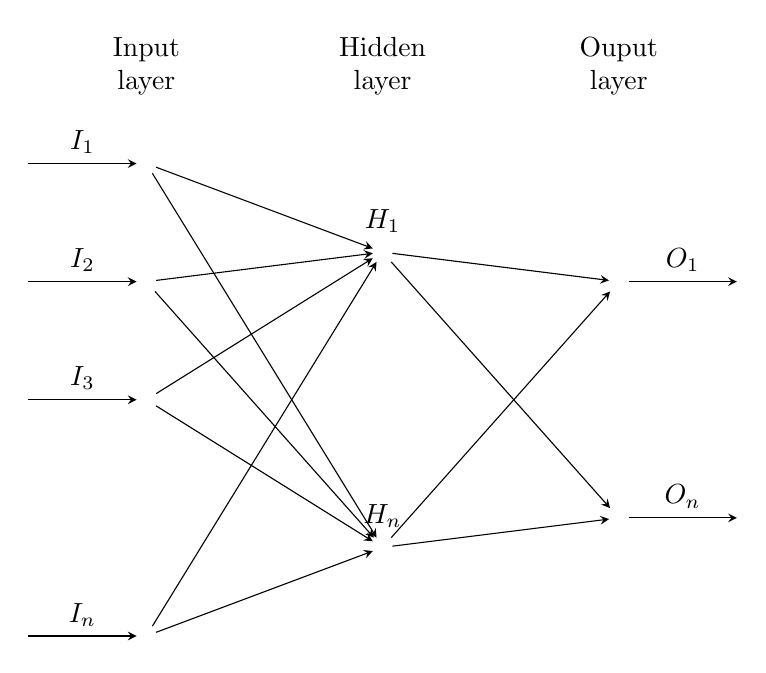
\begin{tikzpicture}[x=1.5cm, y=1.5cm, >=stealth]

\foreach \m/\l [count=\y] in {1,2,3,missing,4}
  \node [every neuron/.try, neuron \m/.try] (input-\m) at (0,2.5-\y) {};
	
\foreach \m [count=\y] in {1,missing,2}
  \node [every neuron/.try, neuron \m/.try ] (hidden-\m) at (2,2-\y*1.25) {};

\foreach \m [count=\y] in {1,missing,2}
  \node [every neuron/.try, neuron \m/.try ] (output-\m) at (4,1.5-\y) {};

\foreach \l [count=\i] in {1,2,3,n}
  \draw [<-] (input-\i) -- ++(-1,0)
    node [above, midway] {$I_\l$};

\foreach \l [count=\i] in {1,n}
  \node [above] at (hidden-\i.north) {$H_\l$};

\foreach \l [count=\i] in {1,n}
  \draw [->] (output-\i) -- ++(1,0)
    node [above, midway] {$O_\l$};

\foreach \i in {1,...,4}
  \foreach \j in {1,...,2}
    \draw [->] (input-\i) -- (hidden-\j);

\foreach \i in {1,...,2}
  \foreach \j in {1,...,2}
    \draw [->] (hidden-\i) -- (output-\j);

\foreach \l [count=\x from 0] in {Input, Hidden, Ouput}
  \node [align=center, above] at (\x*2,2) {\l \\ layer};

\end{tikzpicture}

\subsubsection{Train Network on optdigits}
The Multilayer Neural network is trained on optdigits data with different configurations. Provided corresponding IPython notebook in submission directory. 
\subsubsection{Data}
For this problem as mentioned in the Assignment pdf, the data is downloaded from the UCI Machine Learning Repository. \href{http://archive.ics.uci.edu/ml/machinelearning-databases/optdigits/}{UCI/optdigits}

Using pandas library the training and testing data is loaded into digits and digits test variables respectively.
%%%%%%%%%%%%%%%%%%%%%%%%%%%%%%%%%%%%%%%%%%%%%%%%%%%%%%%%%%%%%%%%%%%%%%%%%%%%%%%%%%%%%%%%%

\lstset{% general command to set parameter(s)
basicstyle=\small, % print whole listing small
identifierstyle=, % nothing happens
stringstyle=\ttfamily, % typewriter type for strings
showstringspaces=false} % no special string spaces

\lstset{language=Python}          % Set your language (you can change the language for each code-block optionally)

\begin{lstlisting}[label=loaddata,caption=Importing the data]  % Start your code-block

digits = pd.read_csv("../datasets/
optdigits/optdigits_train.csv", header=None)

digits_test = pd.read_csv("../datasets/
optdigits/optdigits_test.csv.txt", header=None)

\end{lstlisting}


The dataframes are then converted to matrix type and separated labels, from attributes. 
\graphicspath{ {/images/} }
\begin{figure}[!h]
\includegraphics[scale=0.75]{images/P1/GrayImage.png}
  \caption{Reshaped the data to 8$\times$8}
  \label{fig:grayim}
\end{figure}
\subsubsection{Pre-processing}
The data is reshaped to $8\times8$ to form an image, a sample image is shown in figure \ref{fig:grayim}
%%%%%%%%%%%%%%%%%%%%%%%%%%%%%%%%%%%%%%%%%%%%%%%%%%%%%%%%%%%%%%%%%%%%%%%%%%%%%%%%%%%%%%%%%

\lstset{% general command to set parameter(s)
basicstyle=\small, % print whole listing small
identifierstyle=, % nothing happens
stringstyle=\ttfamily, % typewriter type for strings
showstringspaces=false} % no special string spaces

\lstset{language=Python}          % Set your language (you can change the language for each code-block optionally)

\begin{lstlisting}[label=Image Resize,caption=Array to Image]  % Start your code-block

images = []
size = (8,8)
for x in X_train:
    I = np.resize(x,size)
    images.append(I)
    
# Show a sample image in gray scale

imgs = np.array(images)
imgs.shape
imgs[1]
plt.imshow(imgs[1],cmap='gray')
I1 = imgs[1]
plt.savefig("../Submission/Documentation/images/P1/GrayImage.png")    
\end{lstlisting}

Further the graylevel values are binerized by applying otsu thresholding. The digitized image is shown in figure \ref{fig:binaryim}
    
\graphicspath{ {/images/} }
\begin{figure}[!t]
\includegraphics[scale=0.75]{images/P1/Digitized_Sample_Image.png}
  \caption{Downsampled and Digitized Image}
  \label{fig:binaryim}
\end{figure}


\subsubsection{Classifier}
A multilayer neural network is implemented from scratch,referring the algorithm from DHS Book.
%%%%%%%%%%%%%%%%%%%%%%%%%%%%%%%%%%%%%%%%%%%%%%%%%%%%%%%%%%%%%%%%%%%%%%%%%%%%%%%%%%%%%%%%%
\lstset{% general command to set parameter(s)
basicstyle=\small, % print whole listing small
identifierstyle=, % nothing happens
stringstyle=\ttfamily, % typewriter type for strings
showstringspaces=false} % no special string spaces
\lstset{language=Python}          % Set your language (you can change the language for each code-block optionally)
\begin{lstlisting}[label=activation,caption=Sigmoid Function]  % Start your code-block

# sigmoid function
def sigmoid(x):
    return 1/(1 + np.exp(-x))
   
\end{lstlisting}

%%%%%%%%%%%%%%%%%%%%%%%%%%%%%%%%%%%%%%%%%%%%%%%%%%%%%%%%%%%%%%%%%%%%%%%%%%%%%%%%%%%%%%%%%

\lstset{% general command to set parameter(s)
basicstyle=\small, % print whole listing small
identifierstyle=, % nothing happens
stringstyle=\ttfamily, % typewriter type for strings
showstringspaces=false} % no special string spaces
\lstset{language=Python}          % Set your language (you can change the language for each code-block optionally)
\begin{lstlisting}[label= fwdpass,caption=forward-pass]  % Start your code-block

for x in range(self.X_train.shape[0]):
    a_1 = sigmoid(np.matmul((self.weights1).T, 
    self.X_train[x,:][:,np.newaxis]+self.b1[:,np.newaxis])
        
    a_2 = sigmoid(np.matmul(self.weights2.T, a_1)
    +self.b2[:, np.newaxis])   
   
\end{lstlisting}

%%%%%%%%%%%%%%%%%%%%%%%%%%%%%%%%%%%%%%%%%%%%%%%%%%%%%%%%%%%%%%%%%%%%%%%%%%%%%%%%%%%%%%%%%

\lstset{% general command to set parameter(s)
basicstyle=\small, % print whole listing small
identifierstyle=, % nothing happens
stringstyle=\ttfamily, % typewriter type for strings
showstringspaces=false} % no special string spaces
\lstset{language=Python}          % Set your language (you can change the language for each code-block optionally)
\begin{lstlisting}[label=nh5-testacc,caption=Back-Propagation]  % Start your code-block

# Backpropagation
delta_2 = (a_2 - self.ytrain_OH[x][:, np.newaxis] )*(a_2*(1-a_2))
dE_dw_2 = np.matmul(a_1, delta_2.T)
dE_db_2 = (delta_2)
delta_1 = (a_1*(1-a_1))*np.matmul(self.weights2, delta_2)
dE_dw_1 = np.matmul(self.X_train[x][:,np.newaxis], delta_1.T)             
dE_db_1 = (delta_1)
self.weights1 = self.weights1 - lr_rate*dE_dw_1
self.b1 = self.b1 - lr_rate*dE_db_1[:,0]    
self.weights2 = self.weights2 - lr_rate*dE_dw_2
self.b2 = self.b2 - lr_rate*dE_db_2[:,0]
   
\end{lstlisting}
 

\clearpage
\subsubsection{Report}

%%%%%%%%%%%%%%%%%%%%%%%%%%%%%%%%%%%%%%%%%%%%%%%%%%%%%%%%%%%%%%%%%%%%%%%%%%%%%%%%%%%%%%%%%

\lstset{% general command to set parameter(s)
basicstyle=\small, % print whole listing small
identifierstyle=, % nothing happens
stringstyle=\ttfamily, % typewriter type for strings
showstringspaces=false} % no special string spaces
\lstset{language=Python}          % Set your language (you can change the language for each code-block optionally)
\begin{lstlisting}[label=nh5-testacc,caption=acc on nH=5]  % Start your code-block

mlp125 = MLP(X_train,y_train,125)
print("="*30)
print("Training with 125 hidden units")
print("accuracy")
print("="*30)
mlp125.run()
print("="*30)
print("Prediction accuracy on test data: ")
mlp125.testpredict(X_test,y_test)
print("="*30)
   
\end{lstlisting}

\begin{verbatim}
==============================
Training with 125 hidden units
accuracy
==============================
acc: 0.9682
acc: 0.9871
acc: 0.9940
acc: 0.9940
acc: 0.9974
acc: 0.9983
acc: 0.9983
acc: 0.9983
acc: 0.9983
acc: 0.9991
==============================
Prediction accuracy on test data: 
testpredict()
acc: 0.9926
==============================
\end{verbatim}

\begin{tabular}{|c|c|}
\hline 
Hidden units & Accuracy \\ 
\hline 
5 & 0.9686 \\ 
\hline 
25 & 0.9908 \\ 
\hline 
125 & 0.9926 \\ 
\hline 
250 & 0.9852 \\ 
\hline 
\end{tabular} 
\clearpage
\subsubsection*{Experiments}
Experimented with different Number of Hidden Units as well as learning rates. 

Observations: 
when learning rate increased the network became aggressive and under-performed on test data. 
\begin{verbatim}
==============================
Training with 25 hidden units and learning rate = 1
==============================
acc: 0.3328
acc: 0.5924
acc: 0.4987
acc: 0.5967
acc: 0.6113
acc: 0.5159
acc: 0.5709
acc: 0.5787
acc: 0.5572
acc: 0.5804
==============================
Prediction accuracy on test data: 
testpredict()
acc: 0.5941
==============================
\end{verbatim}

So, choice of the learning rate provides good test accuracy if we choose properly. optimal choice if $\eta = 0.1$
150 Hidden units with learning rate= 0.1 give me a test accuracy of 99\%
\begin{verbatim}
==============================
Training with 25 hidden units
accuracy
==============================
acc: 0.9854
acc: 0.9871
acc: 0.9940
acc: 0.9974
acc: 0.9983
acc: 0.9983
acc: 0.9983
acc: 0.9983
acc: 0.9983
acc: 0.9983
==============================
Prediction accuracy on test data: 
testpredict()
acc: 0.9908
==============================

\end{verbatim}
For higher number of hidden units, the accuracy is falling down sometimes, I suspect we should use optimal number of hidden units for the best model. 
\clearpage

\section{Problem 2}
\subsection{Support Vector Machine}
Support Vector Machines (SVMs) are a family of nice supervised learning algorithms that can train classification and regression models efficiently and with very good performance in practice.\\

The kernel function can be any of the following:\\
linear: $\langle x, x'\rangle$.\\
polynomial: $(\gamma \langle x, x'\rangle + r)^d$. d is specified by keyword degree, r by $coef0$.\\
rbf: $\exp(-\gamma |x-x'|^2). \gamma$ is specified by keyword gamma, must be greater than 0.\\
sigmoid $(\tanh(\gamma \langle x,x'\rangle + r))$, where r is specified by $coef0$.\\

The implementation is based on \href{http://www.csie.ntu.edu.tw/~cjlin/papers/libsvm.pdf}{libsvm}. \\ \href{http://scikit-learn.org/stable/modules/generated/sklearn.svm.SVC.html}{Scikit-Learn} library used to experiment various kernels on given data. 
\subsubsection{Plot the data}
Given data comprises of 199 samples of 2 features, and divided into two classes. pandas library used to read the given csv data file, numpy and matplotlib used to separate into two classes and plotted below\ref{fig:C12T1} .  
\graphicspath{ {/images/} }
\begin{figure}[!h]
\includegraphics[scale=0.75]{images/P2/P2_SVMData_C1C2.png}
  \caption{SVMData}
  \label{fig:C12T1}
\end{figure}
\clearpage
\subsubsection{Polynomial Kernel}
%%%%%%%%%%%%%%%%%%%%%%%%%%%%%%%%%%%%%%%%%%%%%%%%%%%%%%%%%%%%%%%%%%%%%%%%%%%%%%%%%%%%%%%%%

\lstset{% general command to set parameter(s)
basicstyle=\small, % print whole listing small
identifierstyle=, % nothing happens
stringstyle=\ttfamily, % typewriter type for strings
showstringspaces=false} % no special string spaces

\lstset{language=Python}          % Set your language (you can change the language for each code-block optionally)

\begin{lstlisting}[label=loaddata,caption=Importing the data]  % Start your code-block

best_score = 0
k_scores = []
for degree in  [0,1, 2]:
    for C in [0.01,0.01, 0.1, 1, 10,100]:        
        for i in range(1,10):               
            kfold = KFold(n_splits=10)
            svm = SVC(kernel='poly',degree=degree, C=C)
            scores = cross_val_score(svm, X, y, cv=kfold)
        k_scores.append(scores.mean())
#         print("c= {},d={}, scores={}".format(C,degree,max(k_scores)))
        if max(k_scores)>best_score:
            best_score = max(k_scores)
            best_parameters = {'C': C, 'degree': degree}
print('Length of list', len(k_scores))
print('Max of list', max(k_scores))
print("Best score : {:.2f}".format(best_score))
print("Best parameters: ", best_parameters)

\end{lstlisting}

\begin{verbatim}
[output]:
('Length of list', 18)
('Max of list', 0.97499999999999998)
Best score : 0.97
('Best parameters: ', {'C': 100, 'degree': 2})
std: 0.140690078047
\end{verbatim}

\graphicspath{ {/images/} }
\begin{figure}[!h]
\includegraphics[scale=0.75]{images/P2/polyd1c01.png}
  \caption{SVC with polynomia kernel {'C': 0.1, 'degree': 1}}
  \label{fig:poly_ker}
\end{figure}
\clearpage
\subsubsection{RBF Kernel}
%%%%%%%%%%%%%%%%%%%%%%%%%%%%%%%%%%%%%%%%%%%%%%%%%%%%%%%%%%%%%%%%%%%%%%%%%%%%%%%%%%%%%%%%%

\lstset{% general command to set parameter(s)
basicstyle=\small, % print whole listing small
identifierstyle=, % nothing happens
stringstyle=\ttfamily, % typewriter type for strings
showstringspaces=false} % no special string spaces

\lstset{language=Python}          % Set your language (you can change the language for each code-block optionally)

\begin{lstlisting}[label=loaddata,caption=Importing the data]  % Start your code-block

best_score = 0
k_scores = []
k_std = []
for gamma in [0.001, 0.01, 0.1, 1, 10, 100]:
    for C in [0.001, 0.01, 0.1, 1, 10, 100]:        
        for i in range(1,10):               
            kfold = KFold(n_splits=10)
            svm = SVC(kernel='rbf',gamma=gamma, C=C)
            scores = cross_val_score(svm, X, y, cv=kfold)
        k_scores.append(scores.mean())
        k_std.append(scores.std())
#         print("c= {},g={}, scores={}".format(C,gamma,max(k_scores)))
        if max(k_scores)>best_score:
            best_score = max(k_scores)
            best_parameters = {'C': C, 'gamma': gamma}
print('Length of list', len(k_scores))
print('Max of list', max(k_scores))
print("Best score : {:.2f}".format(best_score))
print("Best parameters: ", best_parameters)
print(max(k_std))

\end{lstlisting}

\begin{verbatim}
[output]:
('Length of list', 36)
('Max of list', 0.98000000000000009)
Best score : 0.98
('Best parameters: ', {'C': 100, 'gamma': 1})
standard deviation: 0.139106019872
\end{verbatim}

\graphicspath{ {/images/} }
\begin{figure}[!h]
\includegraphics[scale=0.75]{images/P2/RBFg1c100.png}
  \caption{SVC with RBF kernel {'C': 100, 'gamma': 1}}
  \label{fig:rbf_ker}
\end{figure}
\clearpage%
\subsubsection{Discussion on Performance}
I think the polynomial kernel with provided parameters are performing well than the rbf kernel, as it seems like overfitting the data. 
\\

\begin{tabular}{|c|c|c|c|c|}
\hline 
Kernel & gamma & degree & C & Accuracy\\ 
\hline 
Polynomial & - & 2 & 100 & 0.97\\ 
\hline 
rbf & 1 & - & 100 & 0.98\\ 
\hline 
rbf(validation) & 100 & - & 10 & 0.96\\ 
\hline 
polynomia(val) & - & 2 & 100 & 0.98\\ 
\hline 
\end{tabular} \label{tab1}\\
\\
Hence I have experimented few other combinations of C and gamma for rbf kernel and C and degree for polynomial kernel, and the results are shown in the below section\ref{experiments}.
\clearpage
\subsubsection*{Some Experiments}\label{experiments}
\subsubsection*{best parameters with train, test, validation data}

\graphicspath{ {/images/} }
\begin{figure}[!h]
\includegraphics[scale=0.75]{images/P2/RBFg100c10.png}
  \caption{SVC with RBF kernel {'C': 10, 'gamma': 100}}
  \label{fig:rbf_kerE1}
\end{figure}
\vfill
\clearpage
\subsubsection*{Variations in classification with respect to parameters C, gamma}
\graphicspath{ {/images/} }
\begin{figure}[!h]
\includegraphics[scale=0.75]{images/P2/RBFg10c100.png}
  \caption{SVC with RBF kernel {'C': 100, 'gamma': 10}}
  \label{fig:rbf_kerE2}
\end{figure}

\begin{figure}[!h]
\includegraphics[scale=0.75]{images/P2/RBFg100c100.png}
  \caption{SVC with RBF kernel {'C': 100, 'gamma': 100}}
  \label{fig:rbf_kerE3}
\end{figure}

\vfill
\clearpage
\subsubsection*{Polynomial Kernel and variations in degree,C}
\begin{figure}[!h]
\includegraphics[scale=0.75]{images/P2/polyd2c100.png}
  \caption{SVC with polynomia kernel {'C': 100, 'degree': 2}}
  \label{fig:poly_kerE1}
\end{figure}

\clearpage
%%%%%%%%%%%%%%%%%%%%%%%%%%%%%%%%%%%%%%%%%%%%%%%%%%%%%%%%%%%%%%%%%%%%%%%%%%%%%%%%%%%%%%%%%

\section{Problem 3}
\subsection{ Bayes Decision Theory}
\subsubsection{Data summary}
This data was extracted from the census bureau database found at
\href{http://www.census.gov/ftp/pub/DES/www/welcome.html}{www.census.gov}, and the dataset is contributed to UCI repocitory and freely available at \href{http://archive.ics.uci.edu/ml/machine-learning-databases/census-income-mld/}{census-income-mld} 

 \textbf{Basic statistics for this data set:}\\
 Number of instances data = 199523\\
    Duplicate or conflicting instances : 46716\\
 Number of instances in test = 99762\\
    Duplicate or conflicting instances : 20936\\
    
 \textbf{Class probabilities for income-projected.test file}\\
 Probability for the label '- 50000' : 93.80\%\\
 Probability for the label '50000+' : 6.20\%\\
 Majority accuracy: 93.80\% on value - 50000\\
 Number of attributes = 40 (continuous : 7 nominal : 33)\\
 
The dataset consists of 40 attributes of a mix of nominal as well as continuous data.
%%%%%%%%%%%%%%%%%%%%%%%%%%%%%%%%%%%%%%%%%%%%%%%%%%%%%%%%%%%%%%%%%%%%%%%%%%%%%%%%%%%%%%%%%

\lstset{% general command to set parameter(s)
basicstyle=\small, % print whole listing small
identifierstyle=, % nothing happens
stringstyle=\ttfamily, % typewriter type for strings
showstringspaces=false} % no special string spaces

\lstset{language=Python}          % Set your language (you can change the language for each code-block optionally)

\begin{lstlisting}[label=census-data,caption=loadDataprocess]  % Start your code-block

# load the dataset 
df = pd.read_csv("../datasets/census_income/
census-income-data.csv",header=None)
# show last 5 rows
df.tail()

# remove the duplicate entries
df.drop_duplicates()  

#statistical overview of the data
df.describe()

D= df.as_matrix()
print(D[1])
print("")
print(D.T[-1])

salaryC = D.T[-1]
c1 = np.where(D.T[-1]!=' - 50000.') # which is equal to ' 50000+.'
print(c1)
c2 = np.where(D.T[-1]==' - 50000.')
print(c2)

D1 = D[c1]
D2 = D[c2]
print(D1.shape)
print(D2.shape)

# (12382, 42)
# (183912, 42)
\end{lstlisting}

I read the data, removed duplicate entries and the divided into two classes, One of the samples and the class labels are shown below. 
\begin{verbatim}
"""
[58 ' Self-employed-not incorporated' 4 34 ' Some college but no degree' 0
 ' Not in universe' ' Divorced' ' Construction'
 ' Precision production craft & repair' ' White' ' All other' ' Male'
 ' Not in universe' ' Not in universe' ' Children or Armed Forces' 0 0 0
 ' Head of household' ' South' ' Arkansas' ' Householder' ' Householder'
 1053.55 ' MSA to MSA' ' Same county' ' Same county' ' No' ' Yes' 1
 ' Not in universe' ' United-States' ' United-States' ' United-States'
 ' Native- Born in the United States' 0 ' Not in universe' 2 52 94
 ' - 50000.']

[' - 50000.' ' - 50000.' ' - 50000.' ..., ' - 50000.' ' - 50000.'
 ' - 50000.']
"""
\end{verbatim}

I have also find the unique values within the each column i.e. for each attribute, that helped me figuring out the missing entries correspondence.
%%%%%%%%%%%%%%%%%%%%%%%%%%%%%%%%%%%%%%%%%%%%%%%%%%%%%%%%%%%%%%%%%%%%%%%%%%%%%%%%%%%%%%%%%

\lstset{% general command to set parameter(s)
basicstyle=\small, % print whole listing small
identifierstyle=, % nothing happens
stringstyle=\ttfamily, % typewriter type for strings
showstringspaces=false} % no special string spaces

\lstset{language=Python}          % Set your language (you can change the language for each code-block optionally)

\begin{lstlisting}[label=census-data,caption=missing values]  % Start your code-block

dlist =[]
for col in range(0,41):
    dl = np.unique(df.ix[:,col])
    dlist.append(dl)
    
dlist[27]    
\end{lstlisting}

One of the unique attributes in which we could see a missing value i.e. "?"
\begin{verbatim}
array([' ?', ' Abroad', ' Different county same state',
       ' Different state in Midwest', ' Different state in Northeast',
       ' Different state in South', ' Different state in West',
       ' Nonmover', ' Not in universe', ' Same county'], dtype=object)
\end{verbatim}

%%%%%%%%%%%%%%%%%%%%%%%%%%%%%%%%%%%%%%%%%%%%%%%%%%%%%%%%%%%%%%%%%%%%%%%%%%%%%%%%%%%%%%%%%

\subsubsection{Analysis on mising entries}

\textbf{The principal options for dealing with missing data are.}
\begin{itemize}
\item analysing only the available data (i.e. ignoring the missing data);
\item imputing the missing data with replacement values, and treating these as if they were observed (e.g. last observation carried forward, imputing an assumed outcome such as assuming all were poor outcomes, imputing the mean, imputing based on predicted values from a regression analysis);
\item imputing the missing data and accounting for the fact that these were imputed with uncertainty (e.g. multiple imputation, simple imputation methods (as point 2) with adjustment to the standard error);
\item using statistical models to allow for missing data, making assumptions about their relationships with the available data.
\end{itemize}

I have chosen to replace the missing value with the mode of the column instead removing which leads to huge loss of sample data. 
These are the columns with missing values and their respective modes.\\
\begin{verbatim}
[[21, ' Not in universe'],
 [25, ' Nonmover'],
 [26, ' Nonmover'],
 [27, ' Nonmover'],
 [29, ' Not in universe'],
 [32, ' United-States'],
 [33, ' United-States'],
 [34, ' United-States']]
\end{verbatim}
I wrote my script in such a way that it automatically fetches the missing values and impute them with mode of the column. 

And I found this is one of the research areas. \\
References: \href{https://www.census.gov/srd/csrm/MissingData.html}{Center for Statistical Research and Methodology}

\href{https://liberalarts.utexas.edu/prc/_files/cs/Missing-Data.pdf}{Missing Data \& How to Deal: An
overview of missing data}

I could add them in bibliography but intentionally added here to make them accessible easily, if some one interested in deep digging into the problem. 

\subsubsection{Naive-Bayes in action}
Naive Bayes assumes that the data is independent to each other. So it's called Naive. 
\begin{equation}
P[c|x] = \frac{P[x|c]P(c)}{P(x)}
\end{equation}

In the equation:
$P[c|x]$ is the posterior probability\\
$ P[x|c]$ is the class conditional probability\\
$P(c) , P(x)$ are the prior probabilities\\

IPython notebook is provided in the submission directory. 
After running of 30 iteration on 10 folds the accuracy and the standard deviation as of below.
\begin{verbatim}
acc : 93.7941978907
std : 0.0
\end{verbatim}
%%%%%%%%%%%%%%%%%%%%%%%%%%%%%%%%%%%%%%%%%%%%%%%%%%%%%%%%%%%%%%%%%%%%%%%%%%%
\end{document}
